\section{Galimi kodo skirstymo į paketus šablonai}
Diskusijose, kaip reikėtų skirstyti programinį kodą, paprastai akcentuojami du metodai - pagal \textit{techninį sluoksnį},
kur kiekvienam funkcionalumui arba kompiuterinės sistemos sluoksniui yra sukuriamas paketas,
arba pagal \textit{dalykinės srities esybes}, kur vienos esybės kodas, dalykinės srities
esybės funkcionalumas skirtingose programiniuose sluoksniuose yra patalpintas viename pakete~\cite{PackagingWays}.
Dažniausiai, prioritetas teikiamas kodo skirstymui pagal dalykinės srities esybes~\cite{DomainDrivenDesign} dėl lengvesnio skaitomumo bei
palaikomumo~\cite{DivideByDomain}.
Tačiau šis metodas negali būti vienareikšmiškai pritaikomas kiekvienoje situacijoje ir, dažniausiai praktikoje jo nėra griežtai laikomasi - klasės būna išskaidytos remiantis papildomomis taisyklėmis,
siekiant išspręsti sistemos planavimo metu kylančias problemas.
Norint išskirti šias papildomas taisykles, šablonus, buvo nagrinėjamos atviro kodo sistemos,
stebimi nukrypimai nuo bendresnio kodo skirstymo būdo ir identifikuojami klausimai arba problemos, kurias jais buvo bandoma išspresti.

\subsection{Sistemų analizės procesas}
Praktikoje naudojamų šablonų paieška buvo atliekama stebint atviro kodo sistemų struktūrą ir bandant nustatyti, kodėl pasirenkama nukrypti
nuo pagrindinio skirstymo būdo. Nagrinėtos įvairių tipų sistemos - tiek taikomoji, tiek techninė programinė įranga.
Pastebėta, kad nukrypimai nuo pagrindinio skirstymo būdo dažnai pasikartodavo bandant išspręsti tas pačias problemas,
tačiau jų sprendimo šablonai gali būti skirtingi.

\subsection{Problemos}
Analizuotose sistemose buvo rastos šios problemos, būdingos sistemų dizainui, kartu su jas sprendžiančiais šablonais ir pavyzdžiais,
kokiose sistemose jie yra.

\subsubsection{Pagalbinių, daugkartinio naudojimo klasių skirstymas}
Pagalbinės ir daugkartinio naudojimo klasės dažniausiai negali būti patogiai grupuojamos skirstant pagal dalykinės srities esybes - pagalbines klases gali
naudoti kelios esybės, todėl neaišku, prie kurios jas reikėtų priskirti.
Didžiausia problema, susijusi su pagalbinėmis klasėmis, kurios turėtų išspręsti dažnai sistemoje sutinkamas problemas -
inžinieriai, dirbantys prie sistemos nežino apie jų egzistavimą, todėl jų nenaudoja,
tai veda prie didesnio kodo pasikartojimo arba kelių skirtingų to paties pagalbinio funkcionalumo įgyvendinimų.
\begin{figure}[H]
\snugshade
\dirtree{%
    .1 {/} .
    .2 {users} .
    .3 {UserRolesGrouping} .
    .3 {ArrayGroupingHelper} .
    .2 {\ldots} .
    .2 {payments} .
    .3 {PaymentScheduler} .
    .2 {\ldots} .
    .2 {transactions} .
    .3 {TransactionBatching} .
    .3 {utils} .
    .4 {ArrayGroupByUtil} .
}
\endsnugshade
\caption{Sistemos pavyzdys, kur labai panašią funkciją atliekančios klasės \textit{ArrayGroupByUtil} ir \textit{ArrayGroupingHelper}
egzistuoja todėl, kad inžinierius nerado jau įgyvendintos klasės, dėl aiškios struktūros daugkartinio
panaudojimo klasėms trūkumo.}
\end{figure}
Vienas iš šablonų, sprendžiančių šią problemą, galėtų būti turėti vieną paketą, skirtą visoms pagalbinėmis klasėmis, kuris yra paminėtas sistemos
dokumentacijoje ir apie jo egzistavimą teoriškai žino visi komandos nariai.
Pakete reikėtų turėti atskiras klases kiekvienai bendrinei dalykinei sričiai, iš kurios pavadinimo programuotojas galėtų nuspresti,
kad jo ieškomas funkcionalumas bus būtent toje klasėje.
\begin{figure}[H]
\snugshade
\dirtree{%
    .1 {/} .
    .2 {users} .
    .3 {UserRolesGrouping} .
    .2 {\ldots} .
    .2 {payments} .
    .3 {PaymentScheduler} .
    .2 {\ldots} .
    .2 {transactions} .
    .3 {TransactionBatching} .
    .2 {common} .
    .3 {Arrays} .
    .3 {Maps} .
    .3 {SqlQueries} .
    .3 {Users} .
}
\endsnugshade
\caption{Sistemos pavyzdys, kur visas bendrinio panaudojimo kodas guli \textit{common} pakete, pirmame sistemos paketų lygyje, todėl
pagalbinės klasės yra lengvai randamos.}
\end{figure}
Jei pagalbinių klasių dydis labai išauga, galima vietoje vienos atskiros klasės vienai bendrinei sričiai sukurti vieną paketą,
ir jame turėti kelias pagalbines klases, susijusias su ta dalykine sritimi.
Toks papildomas skirstymo šablonas gali praplėsti skirstymą
pagal dalykinę sritį - jei bendro naudojimo klasės grupuojamos pagal dengiamą sritį, toks skirstymas atitinka bendresnį.
Tokiu atveju reikia užtikrinti, kad iš klasių pavadinimo aišku, kokią smulkesnę dalykinės srities sritį padengia klasė.
\begin{figure}[H]
\snugshade
\dirtree{%
    .1 {/common} .
    .2 {arrays} .
    .3 {ArrayFilters} .
    .3 {ArrayComparators} .
    .2 {\ldots} .
    .2 {maps} .
    .3 {MapTransformations} .
    .3 {MapJoining} .
    .2 {json} .
    .3 {JsonParser} .
    .2 {\ldots} .
    .2 {database} .
    .3 {DatabaseConnection} .
    .3 {DatabaseQueries} .
}
\endsnugshade
\caption{Sistemos pavyzdys, kur bendrinio panaudojimo kodas guli \textit{common} pakete, po dalykinės srities subpaketais, taip sumažinant klasių dydį }
\end{figure}
Tokį pagalbinių klasių skirstymo metodą naudoja keletas repozitorijų - pavyzdžiui, užrašinės aplikacijos \textit{Omni-Notes}\footnote{\url{https://github.com/federicoiosue/Omni-Notes/tree/develop/omniNotes/src/main/java/it/feio/android/omninotes/utils}} bei
\textit{Fire Sticker}\footnote{\url{https://github.com/hackjutsu/Fire_Sticker/tree/master/app/src/main/java/com/gogocosmo/cosmoqiu/fire_sticker/Utils}}.
\textit{Omni-Notes} atveju, \textit{utils} pakete esančios klasės papildomai skirstomos pagal atitinkamą dalykinę sritį.
Naudojant tokį šabloną, programuotojas, susiduriantis su bendrine problema, kuri, labai tikėtina, jau yra išspręsta sistemoje, turėtų
aiškų procesą, kaip elgtis šioje situacijoje:
\begin{enumerate}
    \item Atsidaryti vieną paketą, skirtą bendrinio panaudojimo kodui
    \item Pakete surasti klasę, kurios pavadinimas būtų susijęs su jo problema
    \item Klasės funkcijų saraše surasti jam tinkamą funkciją.
    \item Jei reikalingas funkcionalumas nerastas, įgyvendinti jį pasirinktoje klasėje, padengti jį testais,
    bei aprašyti dokumentaciją, kaip funkcija turėtų būti naudojama.
    \item Iškviesti rastą arba sukurtą funkciją iš bendrinio panaudojimo kodo paketo savo funkcionalume
\end{enumerate}

Šiai problemai spręsti galimas ir kitoks būdas - turėti keletą pagalbinių klasių paketų, patalpintų po atitinkamu bendresniu dalykinės srities
 paketu.
Tokį skirstymo į paketus šabloną naudoja transakcijoms skirta programinė įranga \textit{Seata}\footnote{\url{https://github.com/apache/incubator-seata/tree/2.x/saga/seata-saga-engine/src/main/java/org/apache/seata/saga/engine/utils}}.
Čia pagalbinės klasės yra \textit{utils} pakete žemesniame sistemos lygmenyje, pavyzdžiui, po \textit{engine} paketu.
\begin{figure}[H]
    \snugshade
    \dirtree{%
        .1 {/engine} .
        .2 {strategy} .
        .2 {sequence} .
        .2 {\ldots} .
        .2 {utils} .
        .3 {ExceptionUtils} .
        .3 {\ldots} .
    }
    \endsnugshade
    \caption{Sistemos pavyzdys, kur bendrinio panaudojimo kodas guli \textit{utils} pakete esančiame po dalykinės srities subpaketais}
\end{figure}

\subsubsection{Didelis klasių skaičius pakete}
Sistemai plečiantis, neišvengiamai didėja ir klasių skaičius. Net pasirinkus tinkamą skirstymo klasių skirstymo į paketus metodą
ir palaikant šią tvarką, klasių skaičius pakete gali išaugti. Tokį pavyzdį galima matyti paieškos įrankio \textit{Elasticsearch}\footnote{\url{https://github.com/elastic/elasticsearch/tree/main/server/src/main/java/org/elasticsearch/transport}}
\textit{transport} pakete. Nors klasės yra sugrupuotos pagal dalykinės srities esybę, bendras jų skaičius pakete siekia beveik devyniasdešimt.
Tokiame pakete naviguoti sunku, jis taip pat gali turėti daug priklausomybių.
Jei tokia tendencija yra būdinga visai sistemai, sistema tampa mažiau lanksti pokyčiams, kadangi net ir paprastas pakeitimas
daro įtaką reišmingai sistemos daliai, pokyčiai yra labiau linkę keisti bendrą sistemos architektūrą.
Taip pat naujos sistemos versijos išleidimo \angl{release} procesas tampa sudetingesnis, kadangi yra paveikiama daugiau klasių.
Dažnai matoma, kad susidarius šiai situacijai, nukrypstama nuo skirstymo pagal dalykinės srities esybes, pradedamos grupuoti
techninio sluoksnio klasės. Tokį skirstymą galima matyti \textit{DBeaver} duomenų bazės įrankyje \footnote{\url{https://github.com/dbeaver/dbeaver/tree/devel/plugins/org.jkiss.dbeaver.ext.mssql/src/org/jkiss/dbeaver/ext/mssql}} -
Aukštesniame lygmenyje grupuojant pagal dalykinės srities esybes, pavyzdžiui, \textit{MsSql}, vėliau pereinama prie skirstymo
pagal techninį sluoksnį pakete \textit{model}.
Robert C. Martin bendro sąryšio principas, kuris teigia, kad visos tarpusavyje susijusios klasės turėtų būti vienam pakete,
akcentuoja siekiamybę turėti gan mažus paketus, turinčius aiškiai apibrėžtą funkcionalumą, priežastį egzistuoti, taip užtikrinant ir
glaudų tarpusavyje susijusių klasių saryšį.
Šis principas galėtų būti kodo skirstymo šablonas, užtikrinantis mažesnį klasių bei aferentinių jungčių skaičių paketuose.
Vadovaujantis šiuo šablonu, klases reikėtų skirstyti pagal smulkesnį jų teikiamą funkcionalumą.
Tokį skirstymo tipą galima stebėti \textit{IntelliJ} įskiepyje \footnote{\url{https://github.com/wix-incubator/source-wizard/tree/master/src/main/kotlin/plugin}}.
Čia \textit{plugin} paketo esybė yra papildomai išskirstyta pagal \textit{IntelliJ} sistemos domeno sistemos esybes.
Šį šabloną dar būtų galima patobulinti sprendžiant aferentinių jungčių skaičiaus problemą.
Didelis priklausomybių nuo specifinio paketo skaičius (arba aferentinės jungtys), reiškia, kad pokyčiai tame pakete turės įtaką kelioms klasėms.
Funkcionalumas kitiems paketams galėtų būti pasiekiamas per vieną minimalią sąsają \angl{interface},
kuri atskleidžia tik konceptus (metodus arba duomenų tipus), kurie yra glaudžiai susiję su komponento teikiama paslauga, bei
klase, grąžinančią minėtos sąsajos įgyvendinimą.
Tai gali būti paprasta klasė, su statine funkcija, kurios rezultatas yra ši sąsaja, arba, esant keliomis sąsajos implementacijomis,
\textit{Static factory} dizaino šablonas, kuris nusprendžia, kurį įgyvendinimą reikėtų grąžinti pagal paduotus argumentus.
Visos kitos klasės naudoja \textit{package} pasiekiamumo modifikatorių, taip kompiliatoriaus pagalba užtikrinant,
kad jos nebus pasiektos iš išorės.
Paketas, turintis vieną funkciją, yra naudojamas tik tų paketų, kuriems reikia būtent tos funkcijos,
taip užtikrinant tik mažos sistemos dalies priklausomybę nuo vieno paketo.

Toks principas yra sutinkamas \textit{Typescript} programavimo kalboje, kur kiekvienas modulis (šios kalbos paketo atitikmuo) turi
\textit{index.ts} failą, veikiantį kaip sąsaja, apibrėžianti, kokios modulio klasės bei funkcijos gali būti pasiekiamos už paketo ribų.
Tai užtikrina glaustą kontraktą ir aiškų modulio funkcionalumą, kurį gali pasiekti kiti moduliai, bei paslepia modulio įgyvendinimo detales.
Toki šabloną naudoja turinio valdymo sistema \textit{Keystone}\footnote{\url{https://github.com/keystonejs/keystone/tree/main/packages/core/src/fields/types}},
kur kiekviena esybė turi savo modulį, atliekantį vieną funkciją, kurios kontraktas aprašytas \textit{index.ts} faile.

\begin{figure}[H]
    \snugshade
    \dirtree{%
        .1 {/types} .
        .2 {image} .
        .3 {views} .
        .3 {utils} .
        .3 {index} .
        .2 {text} .
        .3 {views} .
        .3 {index} .
        .2 {...} .
        .2 {checkbox} .
        .3 {views} .
        .3 {index} .
    }
    \endsnugshade
    \caption{\textit{Keystone} sistemos dalis, kurioje matomi smulkūs moduliai su \textit{index.ts} failuose aprašytais kontraktais}
\end{figure}

Taip pat mažas paketo funkcionalumas reiškia, kad minėtas paketas skirtas funkcionalumui įgyvendinti naudos minimalų kitų sistemos esybių skaičių,
taip sumažinant ir eferentinių jungčių skaičių.

Žemiau esančiuose paveikslėliuose galima matyti, kaip išskaidant paketus, turinčius kelis funckionalumus, yra sumažinamas paketų
priklausomybių skaičius.
\begin{figure}[H]
    \centering
    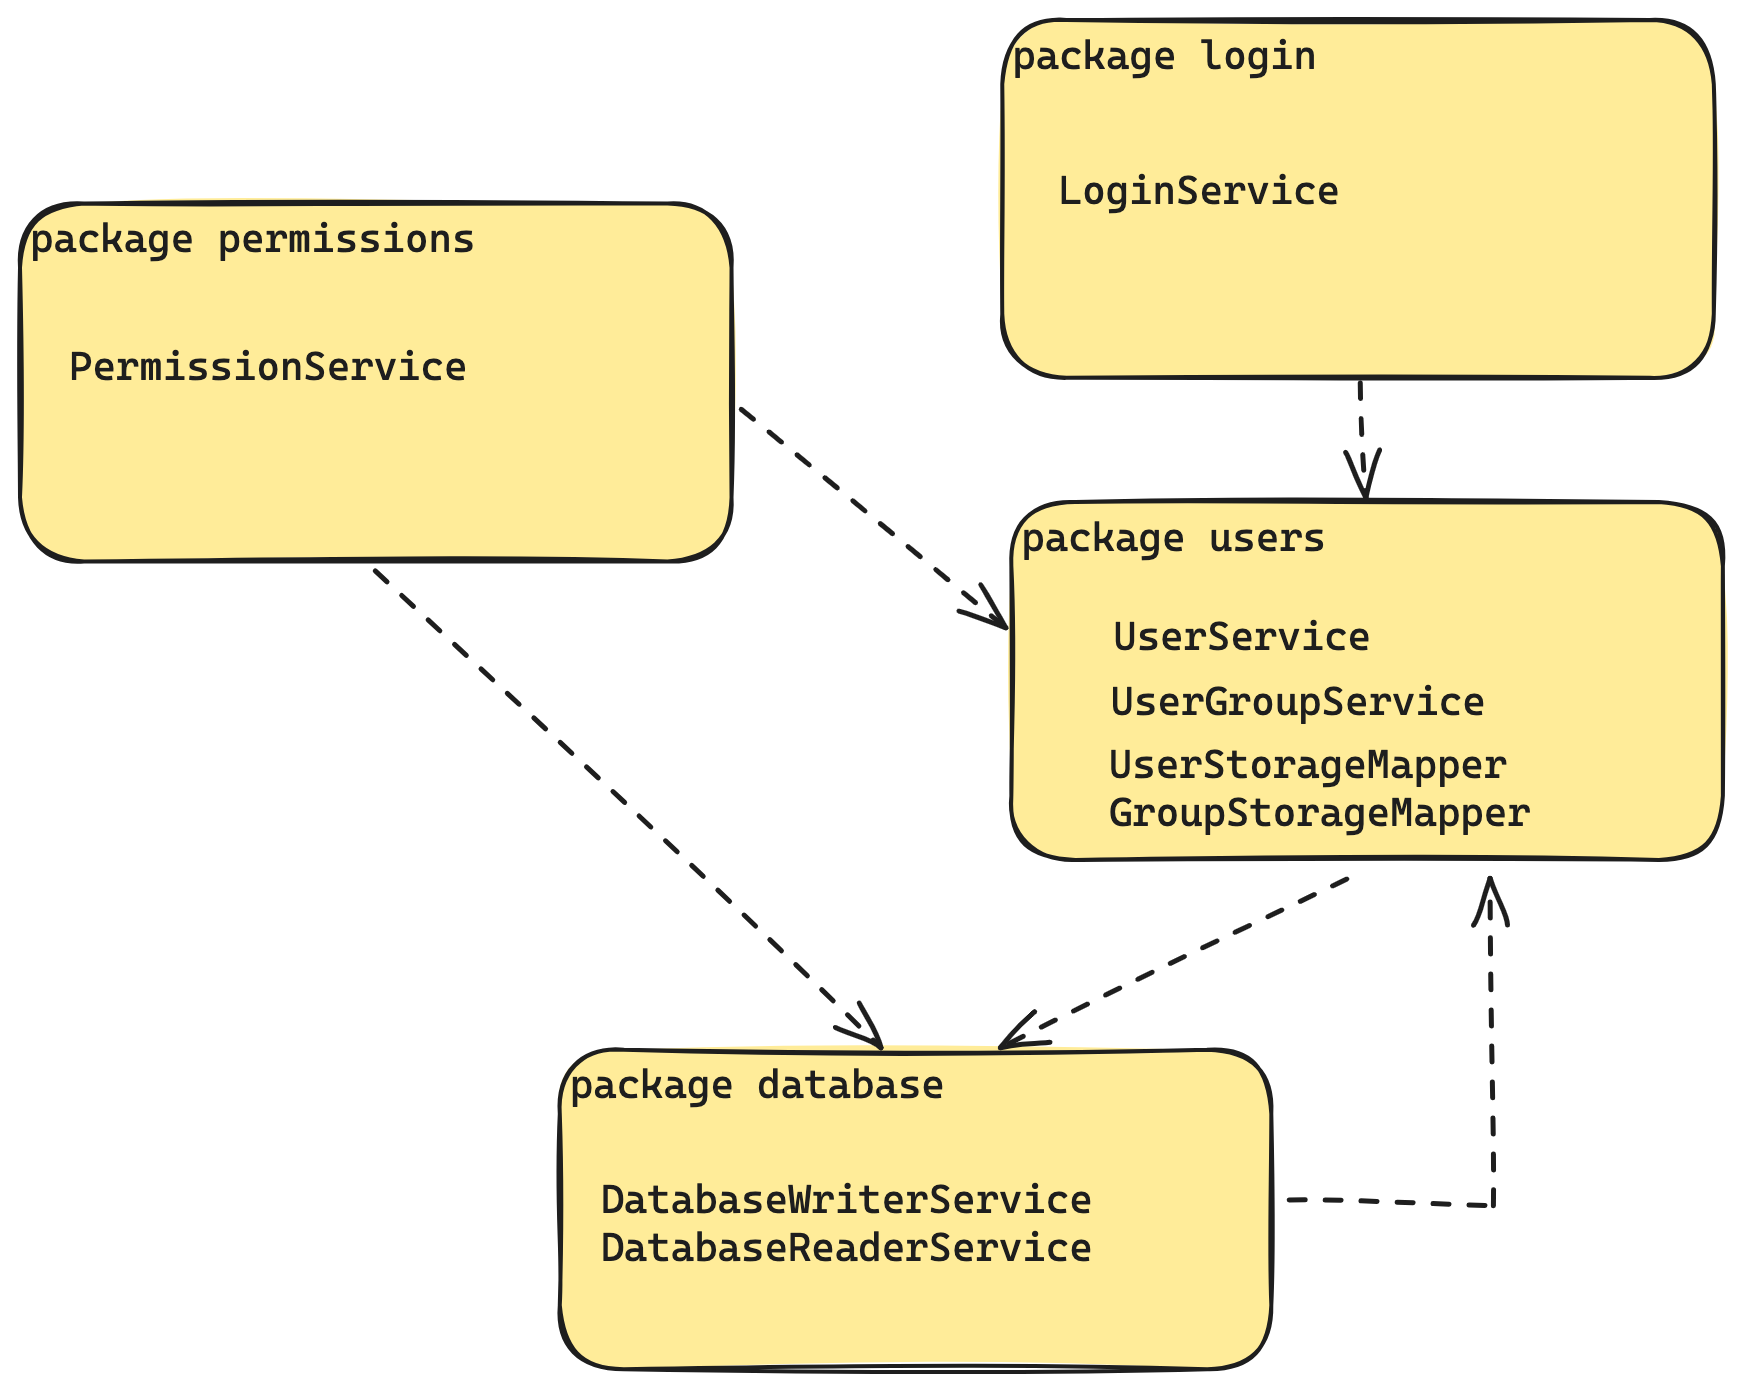
\includegraphics[scale=0.15]{img/excesive_deps}
    \caption{Sistemos pavyzdys su kelias funkcijas atliekančiais paketais}
    \label{img:excesive_deps}
\end{figure}


\begin{figure}[H]
    \centering
    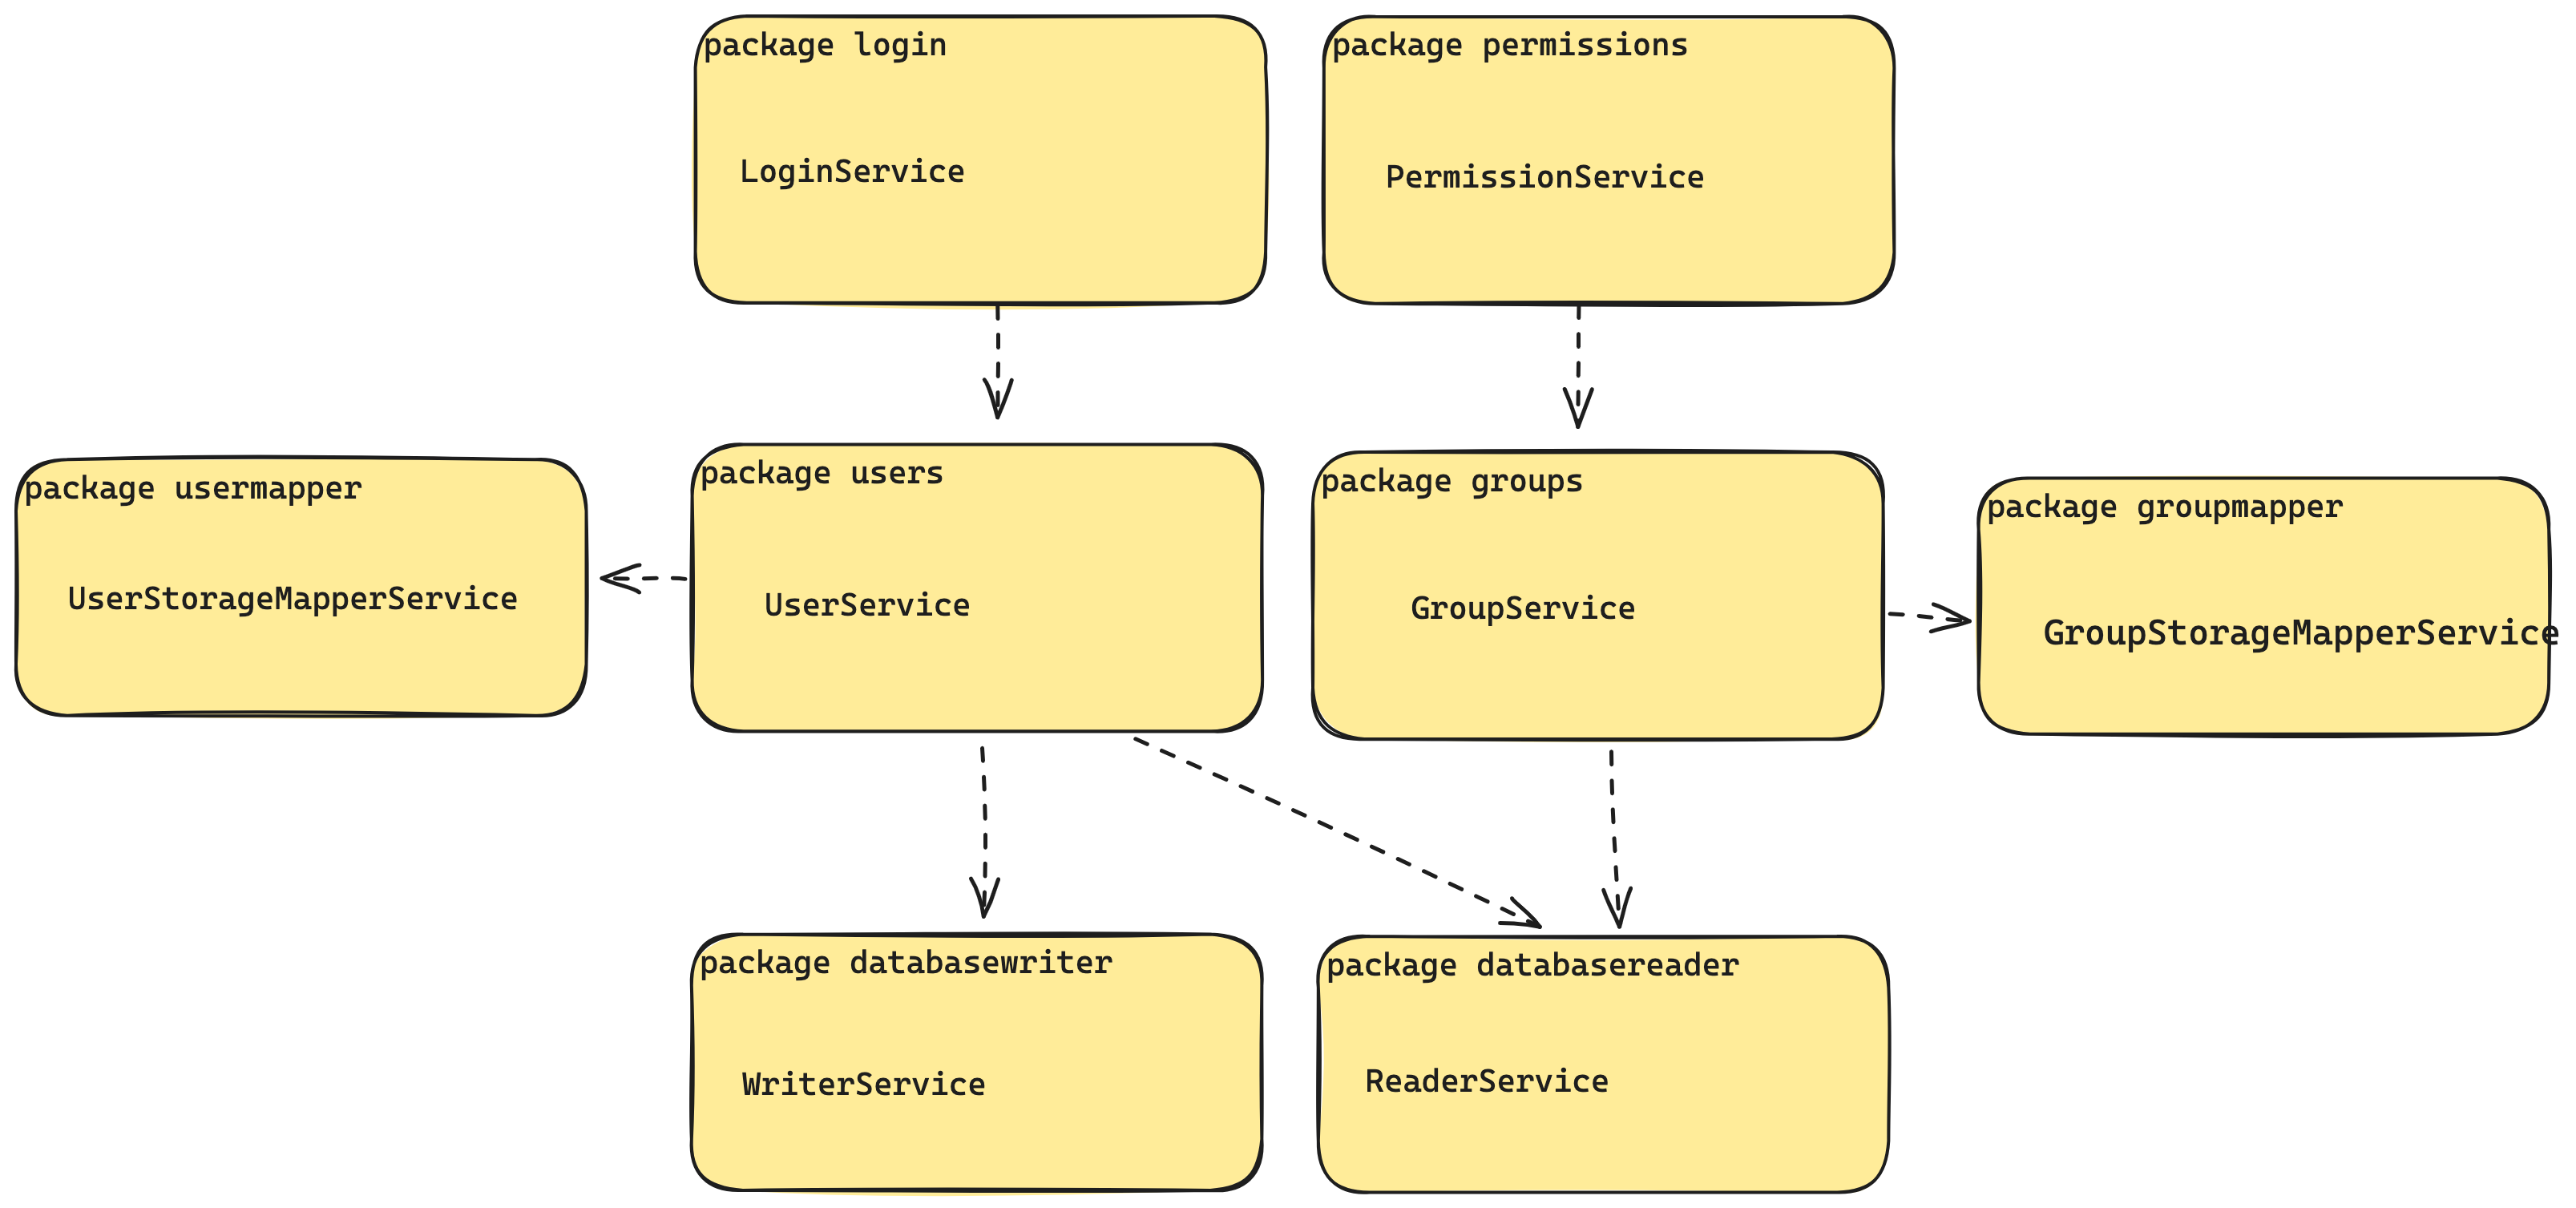
\includegraphics[scale=0.13]{img/good_deps}
    \caption{Sistemos pavyzdys su aiškią, vieną funkciją turinčiais paketais}
    \label{img:good_deps}
\end{figure}

Toks skirstymo būdas taip pat sprendžia ciklinių priklausomybių problemą - pavyzdžiui, įrankio, skirto spręsti ciklinių priklausomybių problemą,
kūrimo aprašas~\cite{CircularDependencies} teigia, kad ciklinių priklausomybių problemą galima spręsti laikantis trijų principų -
bendro panaudojimo, bendro keitimosi bei paleidimo ir pernaudojimo ekvivalentumo.
Šie principai yra išvesti iš bendro saryšio principo ir akcentuoja, kad kartu besikeičiančios klasės turėtų būti viename pakete.
Norint užtikrinti šiuos reikalavimus, reikėtų turėti mažą,
tiksliai apibrėžto funkcionalumo paketą, kurio visi komponentai - tarpusavyje susiję.
Tokiu atveju ciklinių priklausomybių tikimybė sumažėja.

\subsubsection{Daug skirtingų sąsajų implementacijų}
Sistemai plečiantis galima susidurti su problema, kad išauga sąsajos implementacijų skaičius. Ši problema gali iškilti
 skirstant klases pagal dalykinės srities esybes, gali būti neaišku, kur turėtų
būti sukuriamas naujas esybės paketas.
Tokiu atveju navigacija pakete pasidaro sudėtinga, neaišku, kas kurią klasę implementuoja.
Šią problemą galima spręsti sukuriant sąsajos implementacijas tame pačiame pakete kaip ir pati sąsaja.
Toks skirstymo į paketus šablonas yra sutinkamas \textit{Java} standartinėje bibliotekoje\footnote{\url{https://github.com/AdoptOpenJDK/openjdk-jdk11/tree/master/src/java.base/share/classes/java/util}},
kur visos standartinės sąsajos bei jų implementacijos yra tame pačiame pakete.
Dėl tokios paketų struktūros, inžinieriai, naudojantys standartinę \textit{Java} biblioteką, gali lengvai rasti jiems reikiamus sąsajos įgyvendinimus:
\begin{figure}[H]
    \snugshade
    \dirtree{%
        .1 {/util} .
        .2 {Map} .
        .2 {HashMap} .
        .2 {LinkedHashMap} .
        .2 {WeakHashMap} .
        .2 {TreeMap} .
        .2 {...} .
        .2 {List} .
        .2 {LinkedList} .
        .2 {ArrayList} .
    }
    \endsnugshade
    \caption{\textit{Java} standartinės bibliotekos pavyzdys, kuriame sąsajų įgyvendinimai guli tame pačiame pakete, kaip ir sąsajos}
\end{figure}
Šis šablonas turi vieną trūkumą - pakete su dideliu klasių kiekiu, bei keliomis skirtingomis sąsajomis sunku suprasti, kuri klasė kurią sąsają įgyvendina.
Tai pastebima ir \textit{Java} bibliotekos pavyzdyje - \textit{utils} paketas iš viso turi daugiau nei 50 klasių, iš kurių bent 10 yra sąsajos, o visa kita - jų implementacijos,
todėl greitai rasti norimą sąsajos įgyvendinimą vis tiek užtrunka.

Šio šablono trūkumas gali būti išspręstas, jį šiek tiek pakeitus - sąsaja, kuri turi daug skirtingų įgyvendinimų, turėtų turėti specifiškai jai sukurtą paketą, o kiekvienam paketo
įgyvendinimui sukuriamas po subpaketas, kuriame yra tiek klasę įgyvendinanti minėtą sąsają, tiek kitos, įgyvendinimui reikalingos klasės.
Naudojant tokią kodo struktūrą galima labai greitai rasti sąsasas bei galimus jos įgyvendinimus, beveik netyrinėjant sistemos struktūros, bei klasių kodo.
Šis šablonas taip pat užtikrina, kad paketas turi vieną aiškų funkcionalumą, todėl laikosi bendro sąryšio principo.
Šablone aprašyta paketų struktūra buvo sutikta tokiose sistemose kaip \textit{HikariCP}\footnote{\url{https://github.com/brettwooldridge/HikariCP/tree/dev/src/main/java/com/zaxxer/hikari}},
skirtoje efektyviam \textit{Java} programos prisijungimui prie duomenų bazių, bei
\textit{Leaf}\footnote{\url{https://github.com/Meituan-Dianping/Leaf/tree/master/leaf-core/src/main/java/com/sankuai/inf/leaf}}, naudojamoje unikalaus identifikatoriaus generavimui.

\begin{figure}[H]
    \snugshade
    \dirtree{%
        .1 {/} .
        .2 {segment} .
        .3 {dao} .
        .3 {model} .
        .3 {SegmentIdGenImpl} .
        .2 {snowflake} .
        .3 {SnowflakeIdGenImpl} .
        .3 {SnowflakeZookeeperHolder} .
        .2 {IdGen} .
    }
    \endsnugshade
    \caption{\textit{Leaf} sistema, kur kiekvienas sąsajos įgyvendinimas yra aprašytas subpakete}
\end{figure}

\subsubsection{Esybių pokyčių ir versijavimo valdymas}
Sistemai egzistuojant ilgesnį laiką, jos pokyčiai pasidaro neišvengiami.
Smulkūs pokyčiai nebūtinai paveikia bendrą sistemos struktūrą, tačiau
didesniems pokyčiams kartais reikia sukurti naujas klasių ar funkcionalumų versijas. Jei reikia palaikyti atgalinį
suderinamumą (angl. backward compatibility), sistemoje gali atsirasti kelios tų pačių esybių versijos.
Tokiu atveju sistemoje egzistuojančios kelios tų pačių esybių versijos gali pridėti painumo.
Ši problema dažnai sprendžiama sukuriant atskirus paketus skirtingoms
versijoms (v1, v2, v3, \ldots) bei iškeliant bendrą, abiejų esybių naudojamą kodą į paketus taip, kad jas galėtų pasiekti abi versijos.
Taip galima išvengti kodo duplikacijos bei perteklinio klasių skaičiaus paketuose, bei užtikrinant aiškią skirtingų versijų
atskirtį. Toks skirstymas gali praplėsti skirstymą pagal dalykinės srities esybes - skirstomos versijos gali atspindėti reikalingus
palaikyti besikeičiančius verslo reikalavimus.
\begin{figure}[H]
    \snugshade
    \dirtree{%
        .1 {/regex} .
        .2 {common} .
        .2 {pending} .
        .2 {v3} .
        .2 {v4} .
        .2 {...} .
    }
    \endsnugshade
    \caption{\textit{Mongo} duomenų bazės pavyzdys, kuriame skirtingos versijos patalpintos atskiruose paketuose}
\end{figure}
Toks skirstymo būdas matomas keliose repozitorijose - \textit{Mongo}\footnote{\url{https://github.com/mongodb/mongo/tree/master/src/third_party/boost/boost/regex}} duomenų bazėje,
API skirtame kelionių valdymui \textit{travels-java-api}\footnote{\url{https://github.com/mariazevedo88/travels-java-api/tree/master/src/main/java/io/github/mariazevedo88/travelsjavaapi/controller}}
 bei duomenų saugojimo įrankyje \textit{nocodb}\footnote{\url{https://github.com/nocodb/nocodb/tree/c7cc1f92fd77f8b5daefceb7148aab4a69cb9b4e/packages/nocodb/src/meta/migrations}}.
Šiose repozitorijose v1, v2 pavadinti paketai saugo skirtingas esybių versijas.

Apibendrinant, galima išskirti aukščiau aprašytus šablonus:
\begin{center}
    \begin{tabular}{|p{5cm}|p{10cm}|}
        \hline
        Šablonas &  Pavadinimas \\ [0.5ex]
        \hline\hline
        Sprendžiama problema & Pagalbinių klasių skirstymas\\
        \hline
        Siūlomas sprendimas & Sukurti atskirą pagalbinių klasių paketą dalykinės srities esybių lygmenyje \\
        \hline
        Galimos variacijos & Gali būti papildomai sukuriami subpaketai pagal pagalbinių klasių dengiamą funkcionalumą \\
        \hline
    \end{tabular}
    \begin{tabular}{|p{5cm}|p{10cm}|}
        \hline
        Šablonas &  Pavadinimas \\ [0.5ex]
        \hline\hline
        Sprendžiama problema & Pagalbinių klasių skirstymas\\
        \hline
        Siūlomas sprendimas & klases laikyti \textit{util} paketuose, žemesniame lygmenyje nei dalykinės srities esybės \\
        \hline
    \end{tabular}
    \begin{tabular}{|p{5cm}|p{10cm}|}
        \hline
        Šablonas &  Pavadinimas \\ [0.5ex]
        \hline\hline
        Sprendžiama problema & Didelis klasių skaičius pakete\\
        \hline
        Siūlomas sprendimas & klases suskirstyti pagal smulkesnį jų teikiamą funkcionalumą \\
        \hline
        Galimos variacijos & Smulkūs moduliai su atskirose klasėse aprašytais kontraktais \\
        \hline
    \end{tabular}
    \begin{tabular}{|p{5cm}|p{10cm}|}
        \hline
        Šablonas &  Pavadinimas \\ [0.5ex]
        \hline\hline
        Sprendžiama problema & Daug skirtingų sąsajų implementacijų\\
        \hline
        Siūlomas sprendimas & Kiekvienam paketo įgyvendinimui sukurti subpaketą, kuriame yra tiek klasę įgyvendinanti sąsaja, tiek kitos, įgyvendinimui reikalingos klasės \\
        \hline
    \end{tabular}
    \begin{tabular}{|p{5cm}|p{10cm}|}
        \hline
        Šablonas &  Pavadinimas \\ [0.5ex]
        \hline\hline
        Sprendžiama problema & Esybių pokyčių ir versijavimo valdymas\\
        \hline
        Siūlomas sprendimas & Sukurti atskirus paketus skirtingoms versijoms bei iškelti bendrą, abiejų esybių naudojamą kodą į paketus \\
        \hline
    \end{tabular}

\end{center}

